\documentclass[superscriptaddress,onecolumn,floatfix]{revtex4-2}

\usepackage{graphicx}
\usepackage{epsfig}
\usepackage{color}
\usepackage{amssymb}
\usepackage{amsmath}
\usepackage{array}
\usepackage[loose]{units}
\usepackage{hyperref}
\usepackage{cleveref}
\usepackage{braket}
\usepackage[caption=false]{subfig}
\usepackage[english]{babel}
\usepackage{letltxmacro}

\LetLtxMacro{\ORIGselectlanguage}{\selectlanguage}
\makeatletter
\DeclareRobustCommand{\selectlanguage}[1]{%
    \@ifundefined{alias@\string#1}
      {\ORIGselectlanguage{#1}}
      {\begingroup\edef\x{\endgroup
         \noexpand\ORIGselectlanguage{\@nameuse{alias@#1}}}\x}%
}
\newcommand{\definelanguagealias}[2]{%
  \@namedef{alias@#1}{#2}%
}
\makeatother

\definelanguagealias{en}{english}


\begin{document}
                            
\begin{abstract}
  This guide walks you through the steps needed to change the mode of your head unit man-in-the-middle (MITM) harness between MITM and parallel modes. This is a troubleshooting or advanced DIY step. See also the \href{https://youtu.be/sWzxWfUpCfs}{video guide}.
\end{abstract}
\title{Head unit man-in-the-middle mode swap guide}
\author{Electroniq Buttons Boutique}
\email{support@electroniqbuttons.com}
% \affiliation{\GOE}
% \author{Benjamin J. McMorran}
% \email{mcmorran@uoregon.edu}
% \affiliation{\UO}
\date{\today}

\maketitle

\section{Introduction}
The head unit man-in-the-middle (MITM) harness, shown in Figure \ref{subfig:overview:harness}, has two possible modes:
\begin{enumerate}
  \item man-in-the-middle, or serial \label{enum:MITM}
  \item parallel \label{enum:parallel}
\end{enumerate}
\begin{figure}[h]
  \subfloat[]{\label{subfig:overview:harness}
  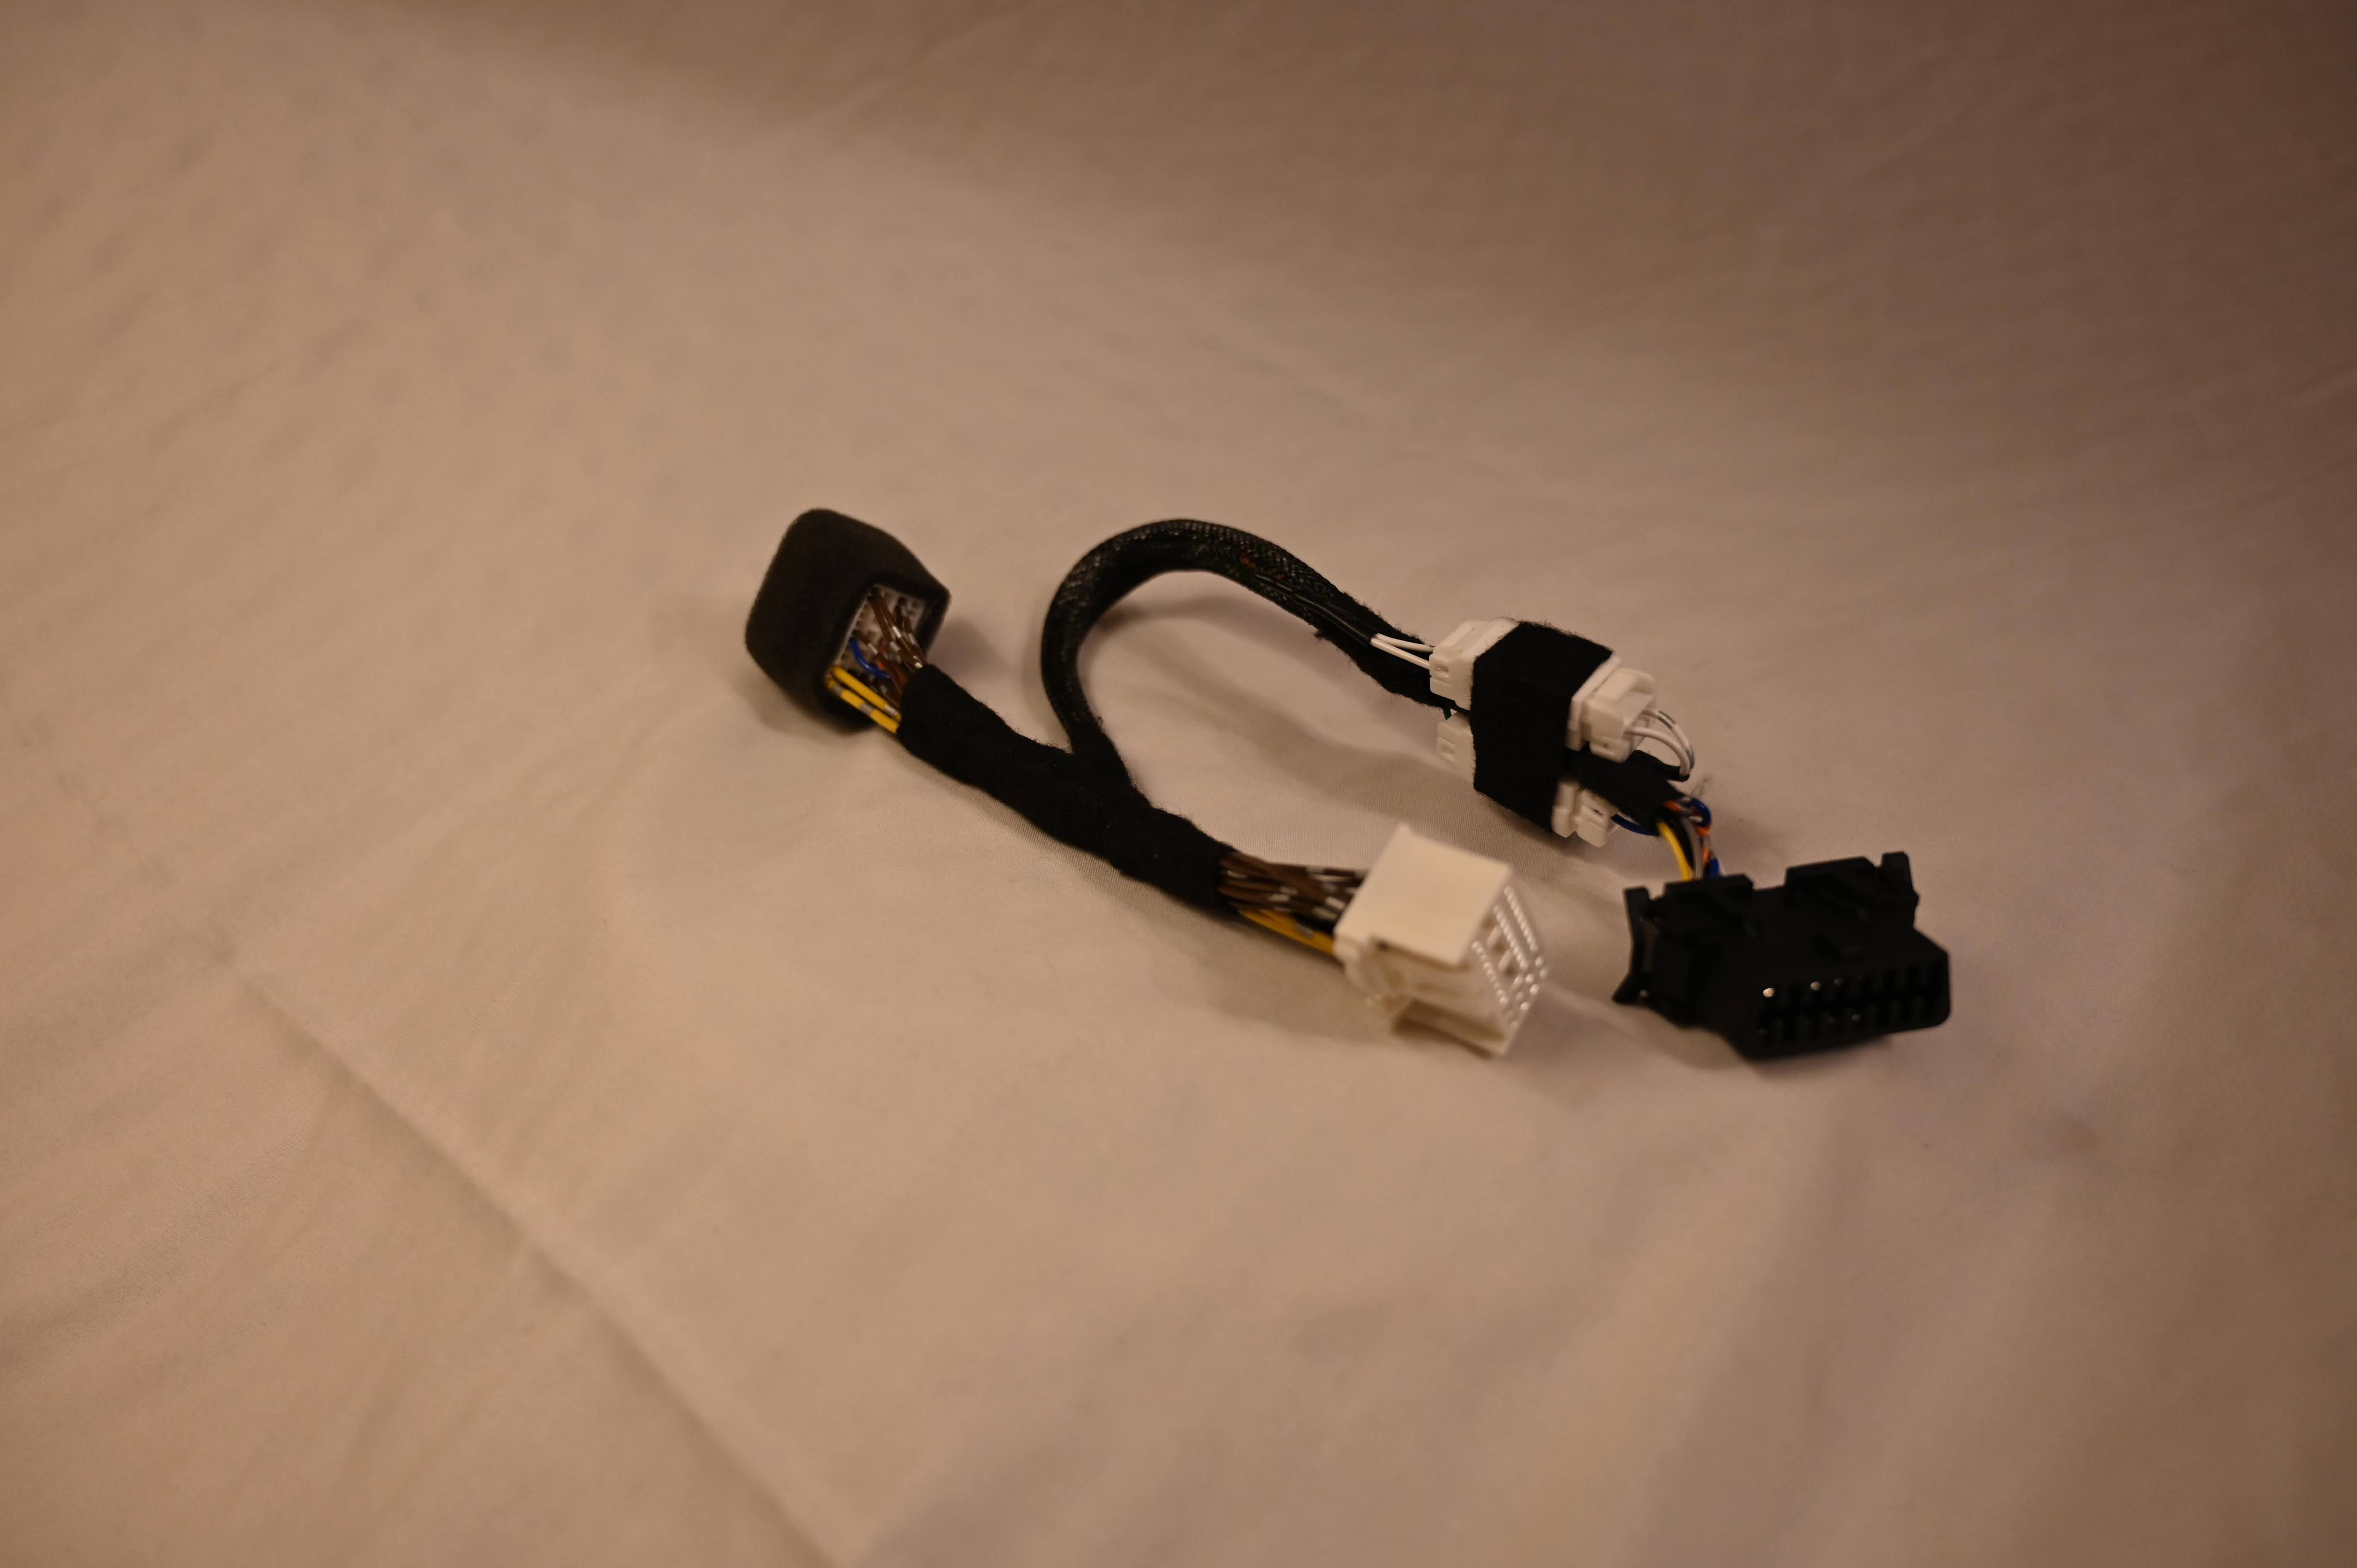
\includegraphics[height=1.95in]{photos/whole_harness.jpg} }
  \subfloat[]{\label{subfig:overview:shunt_cap_labeled}
  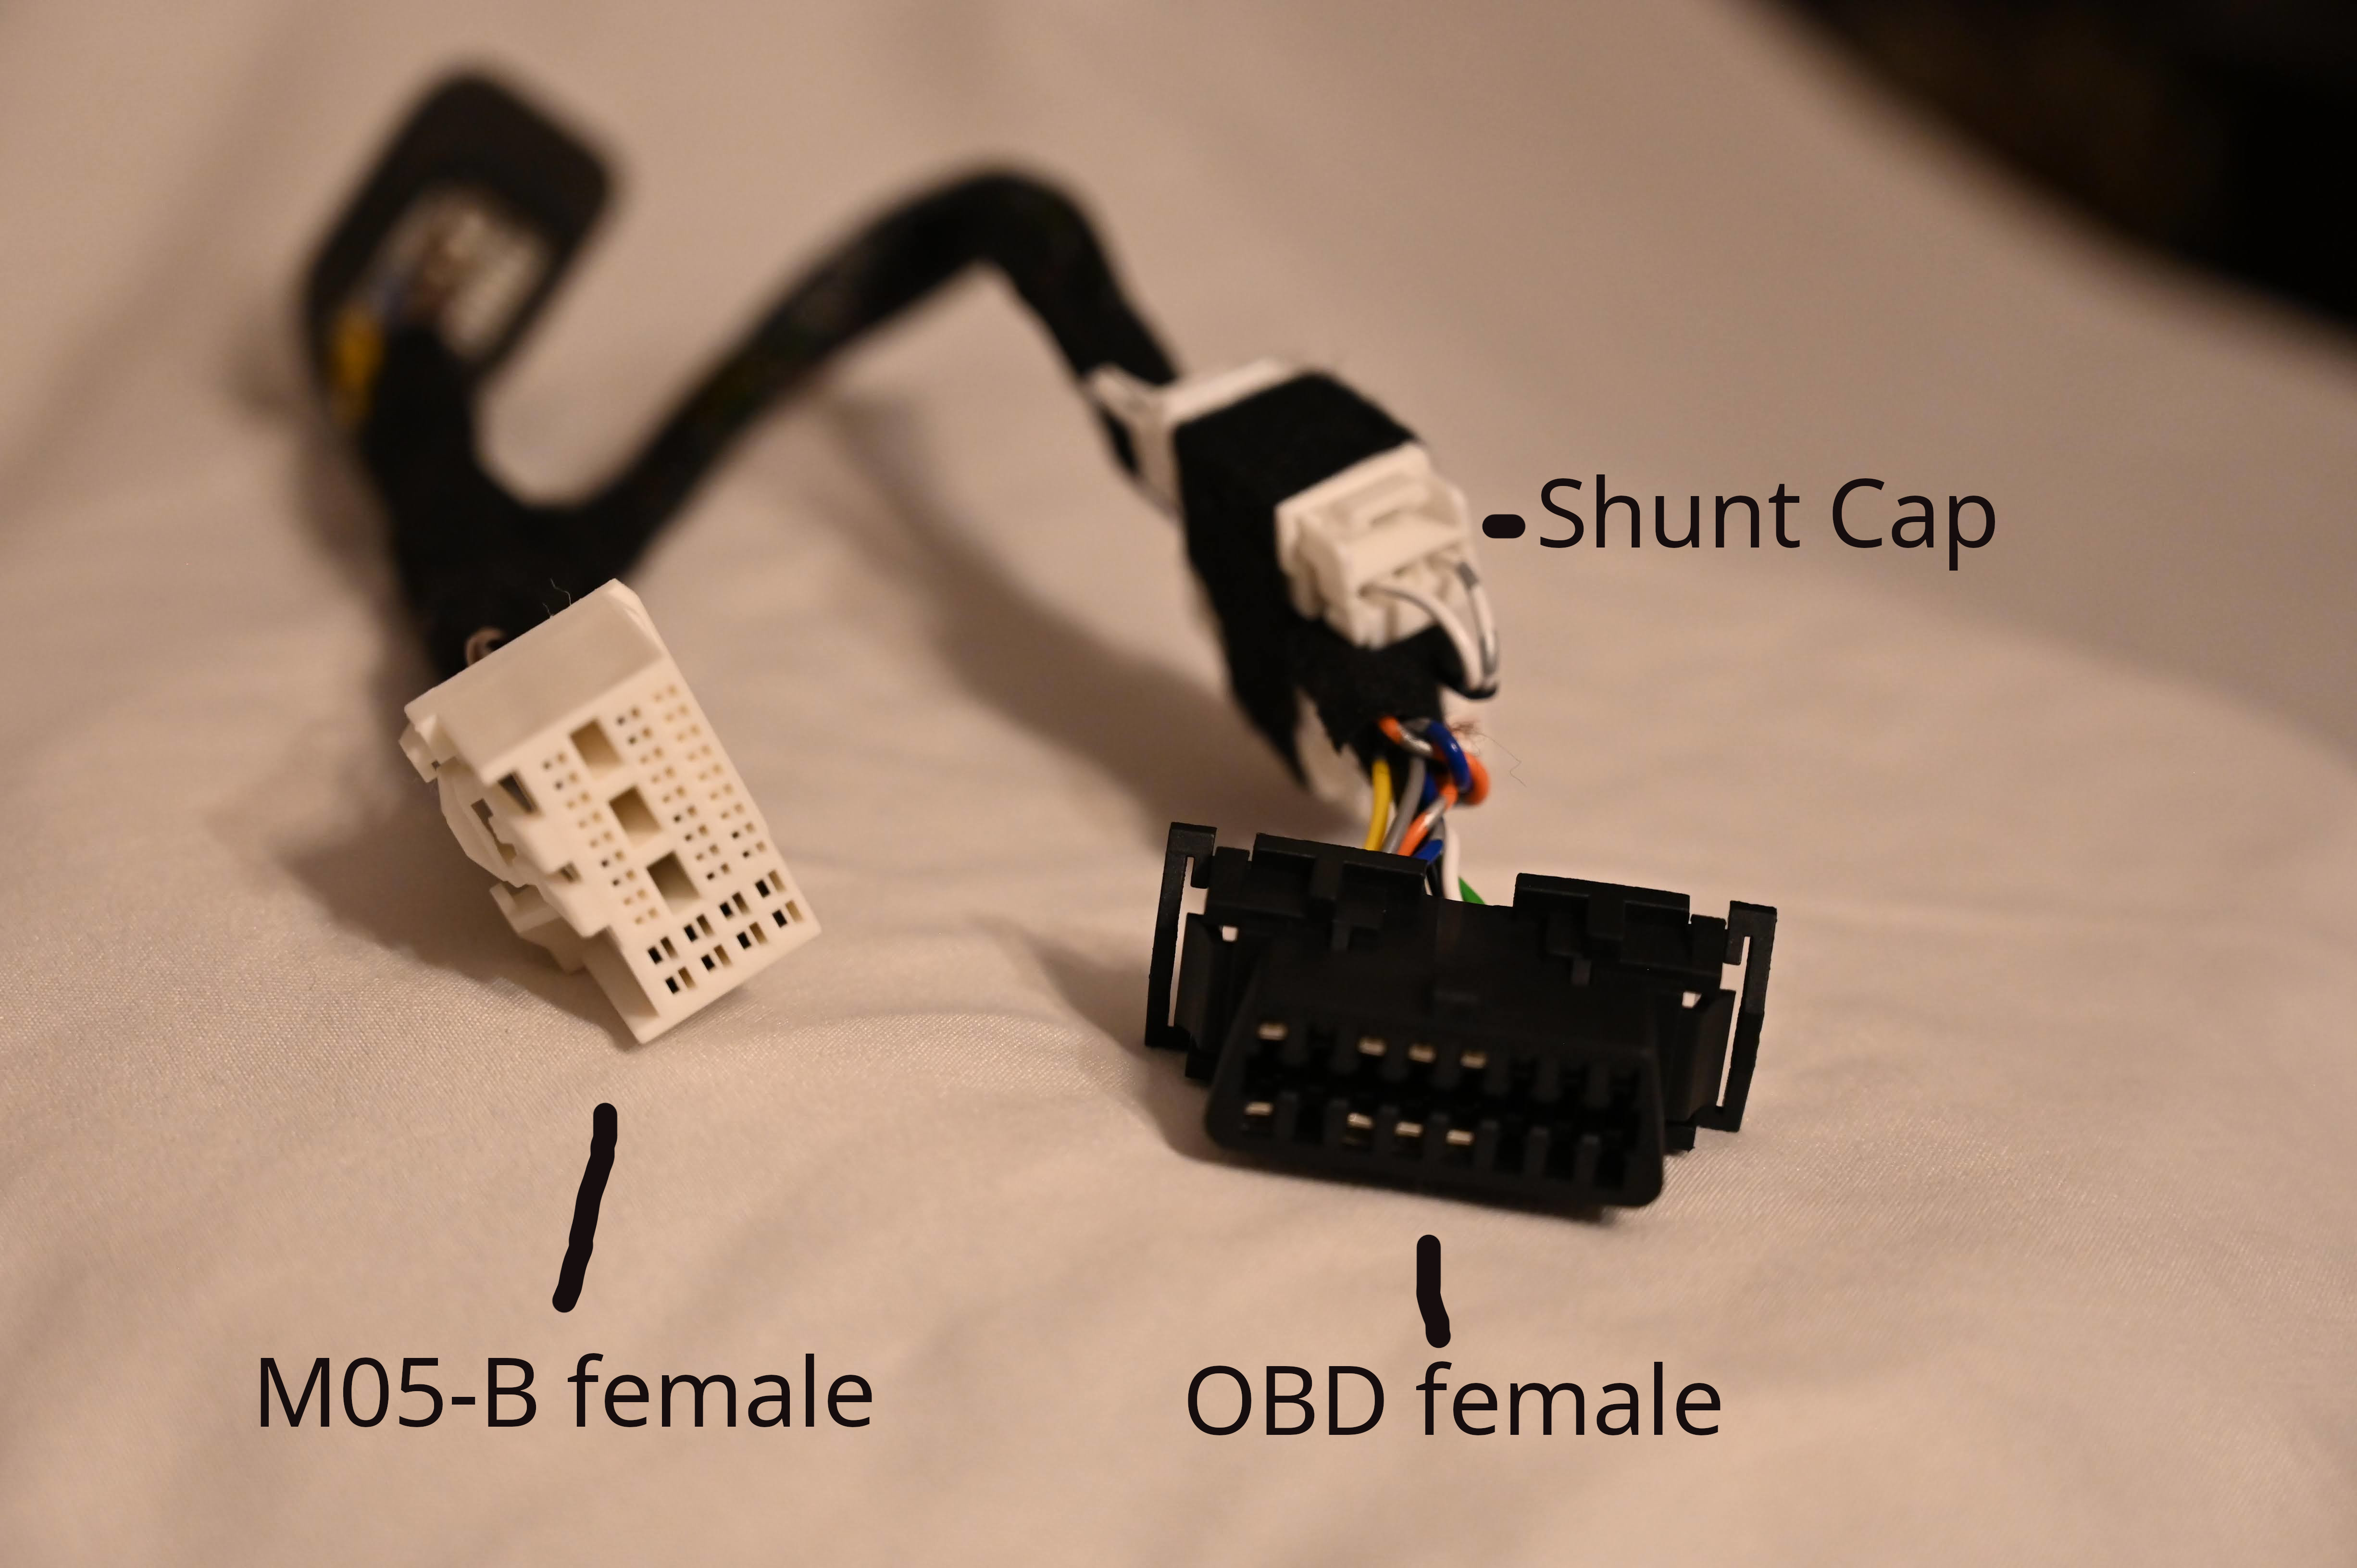
\includegraphics[height=1.95in]{photos/labeled_connectors_MITM_harness.jpg} }
   \caption{(a) Man-in-the-middle harness. (b) Overview of connectors showing shunt cap. \label{fig:overview}}
\end{figure}
In man-in-the-middle mode, the CAN communication lines for the head unit and car are physically disconnected, and a microcontroller plugged into the OBD port is used to selectively pass messages between the two. In parallel mode, the CAN communication lines are connected normally and both CAN pin sets on the OBD port are identical and connected to both the car and head unit. The microcontroller sits on the CAN bus in the same way that a lot of ECUs are connected: in parallel, able to send and receive messages that are shared with all ECUs on the bus. 

The harness is designed to be used primarily in MITM mode, but parallel mode is provided for several reasons:
\begin{enumerate}
  \item troubleshooting
  \item compatibility
\end{enumerate}
If, for example, the MITM ever fails, you can easily switch to parallel mode and continue to use your head unit normally without de-installing the harness. In addition, some microcontrollers only have one CAN pin set and cannot do forwarding. Parallel mode is provided for compatibility in these cases.

\section{How to switch}
To switch, you just have to swap the female shunt and shunt caps, which sit closest to the OBD port. To move from MITM to parallel, do the following:
\begin{enumerate}
  \item Check that current harness mode is MITM (Figure \ref{subfig:shunt:MITM})
  \item Disconnect the female shunt (orange and blue wires, labeled "B1") (Figure \ref{subfig:shunt:female_disconnect})
  \item Disconnect the female shunt cap (white wires, labeled "A2") (Figure \ref{subfig:shunt:cap_removed})
  \item Connect the female shunt into the male shunt (green and white wires, labeled "A1") (Figure \ref{subfig:shunt:parallel})
  \item Connect the female shunt cap into the male shunt cap (white wires, labeled "B2") (Figure \ref{subfig:shunt:parallel})
\end{enumerate}
To reverse the mode, just reverse these instructions!
\begin{figure}[h]
  \subfloat[]{\label{subfig:shunt:MITM}
  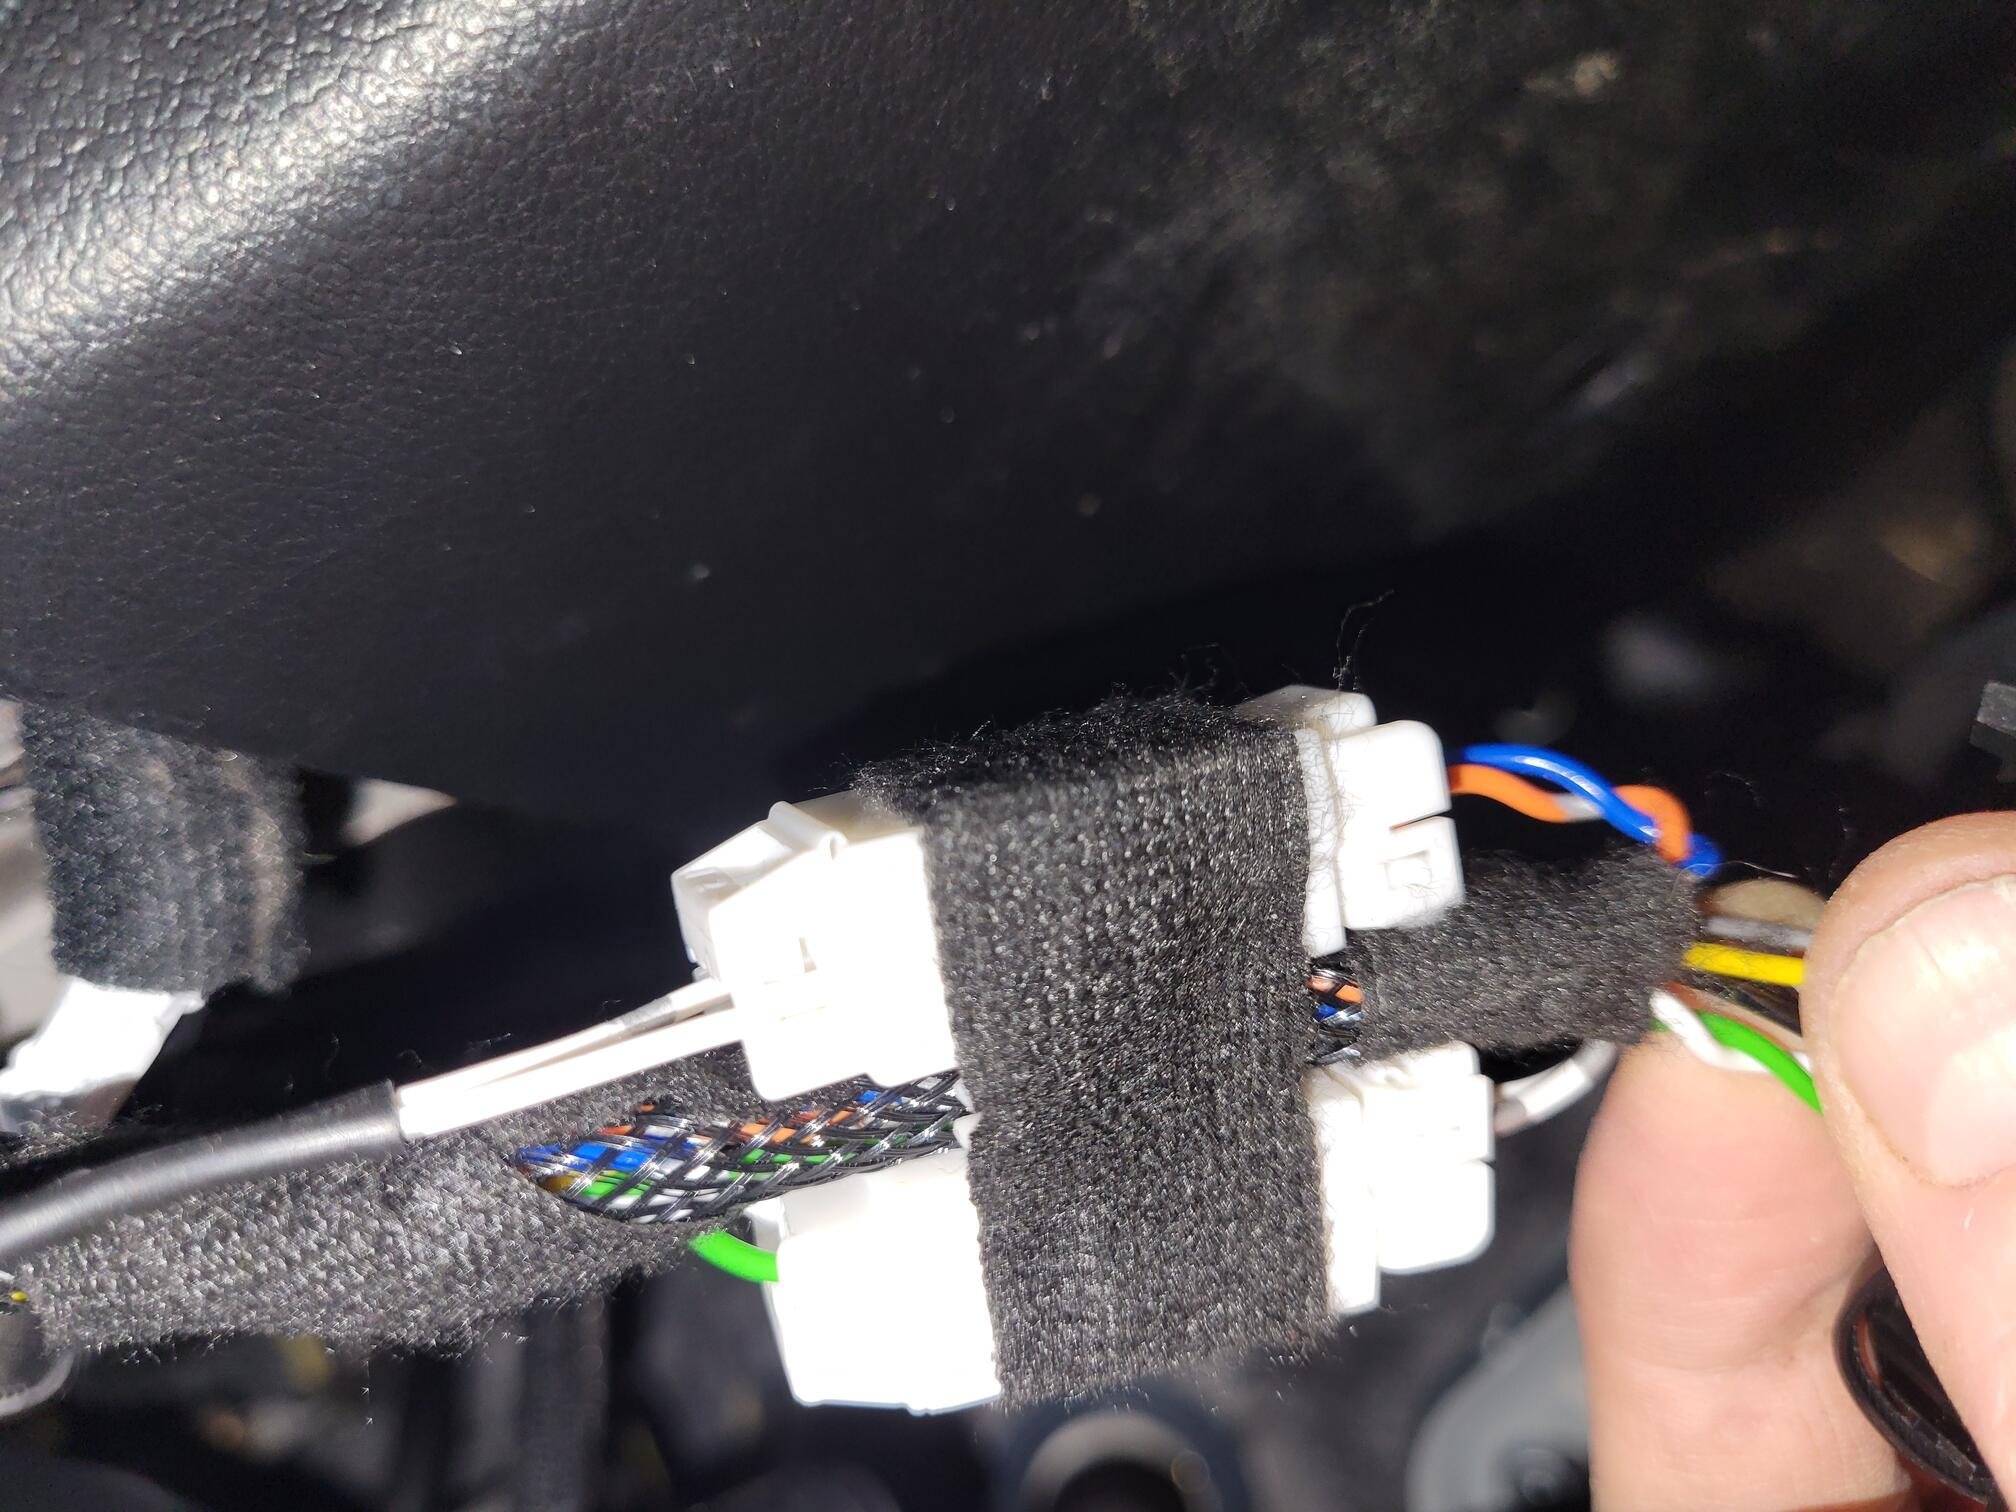
\includegraphics[height=0.95in]{photos/MITM.jpg} }
  \subfloat[]{\label{subfig:shunt:female_shunt_in_cap}
  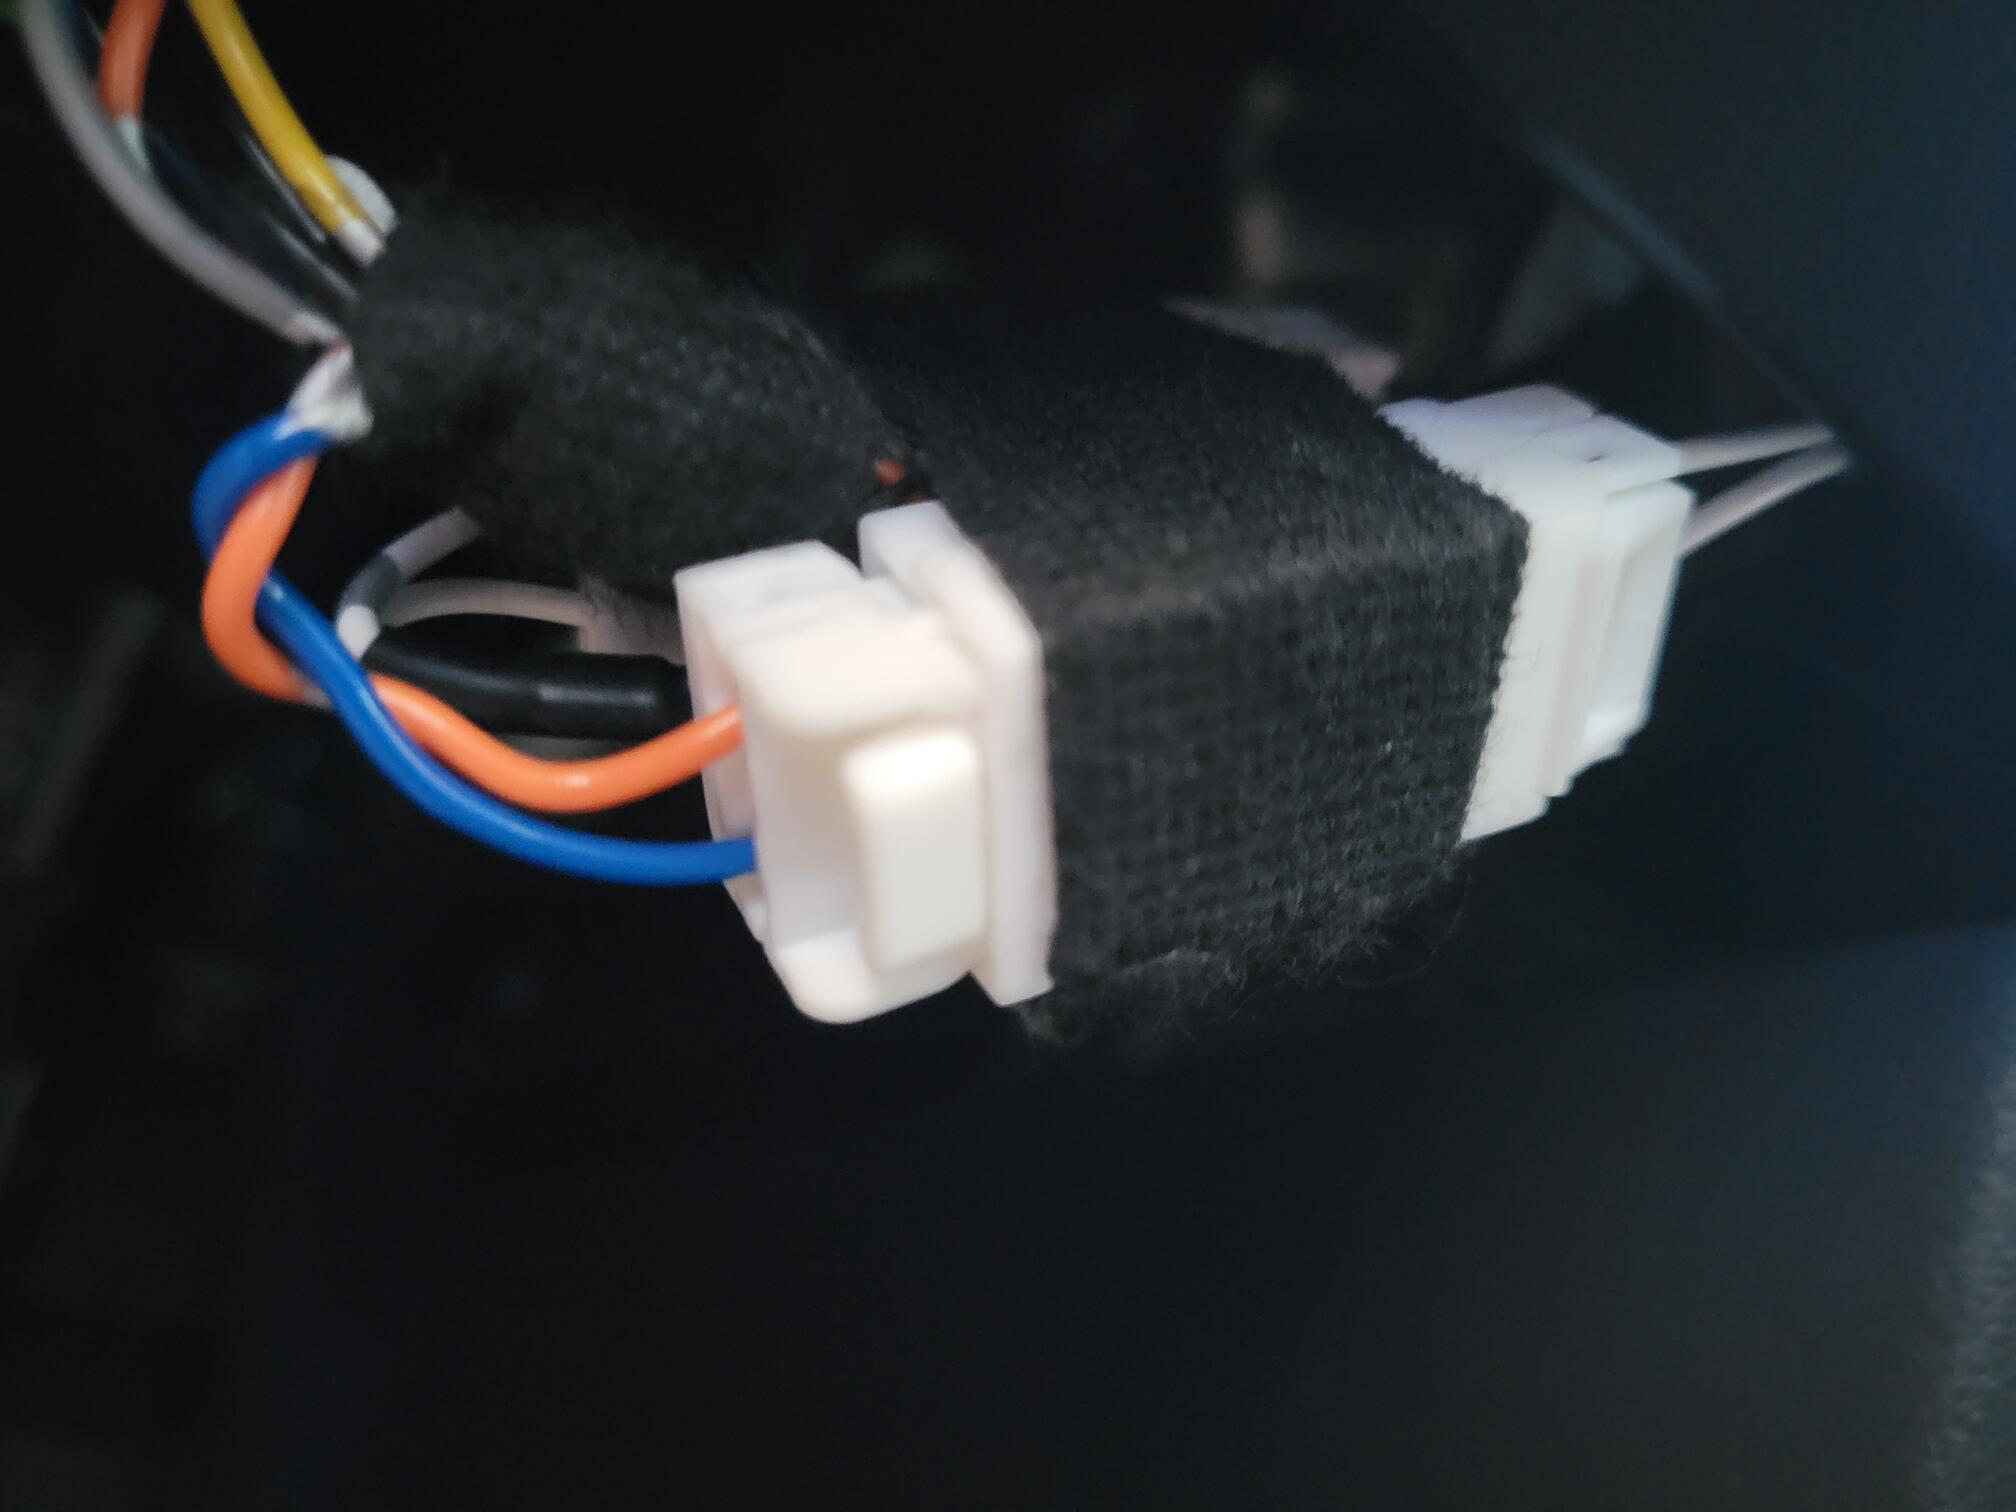
\includegraphics[height=0.95in]{photos/female_shunt_in_shunt_cap.jpg} }
  \subfloat[]{\label{subfig:shunt:female_disconnect}
  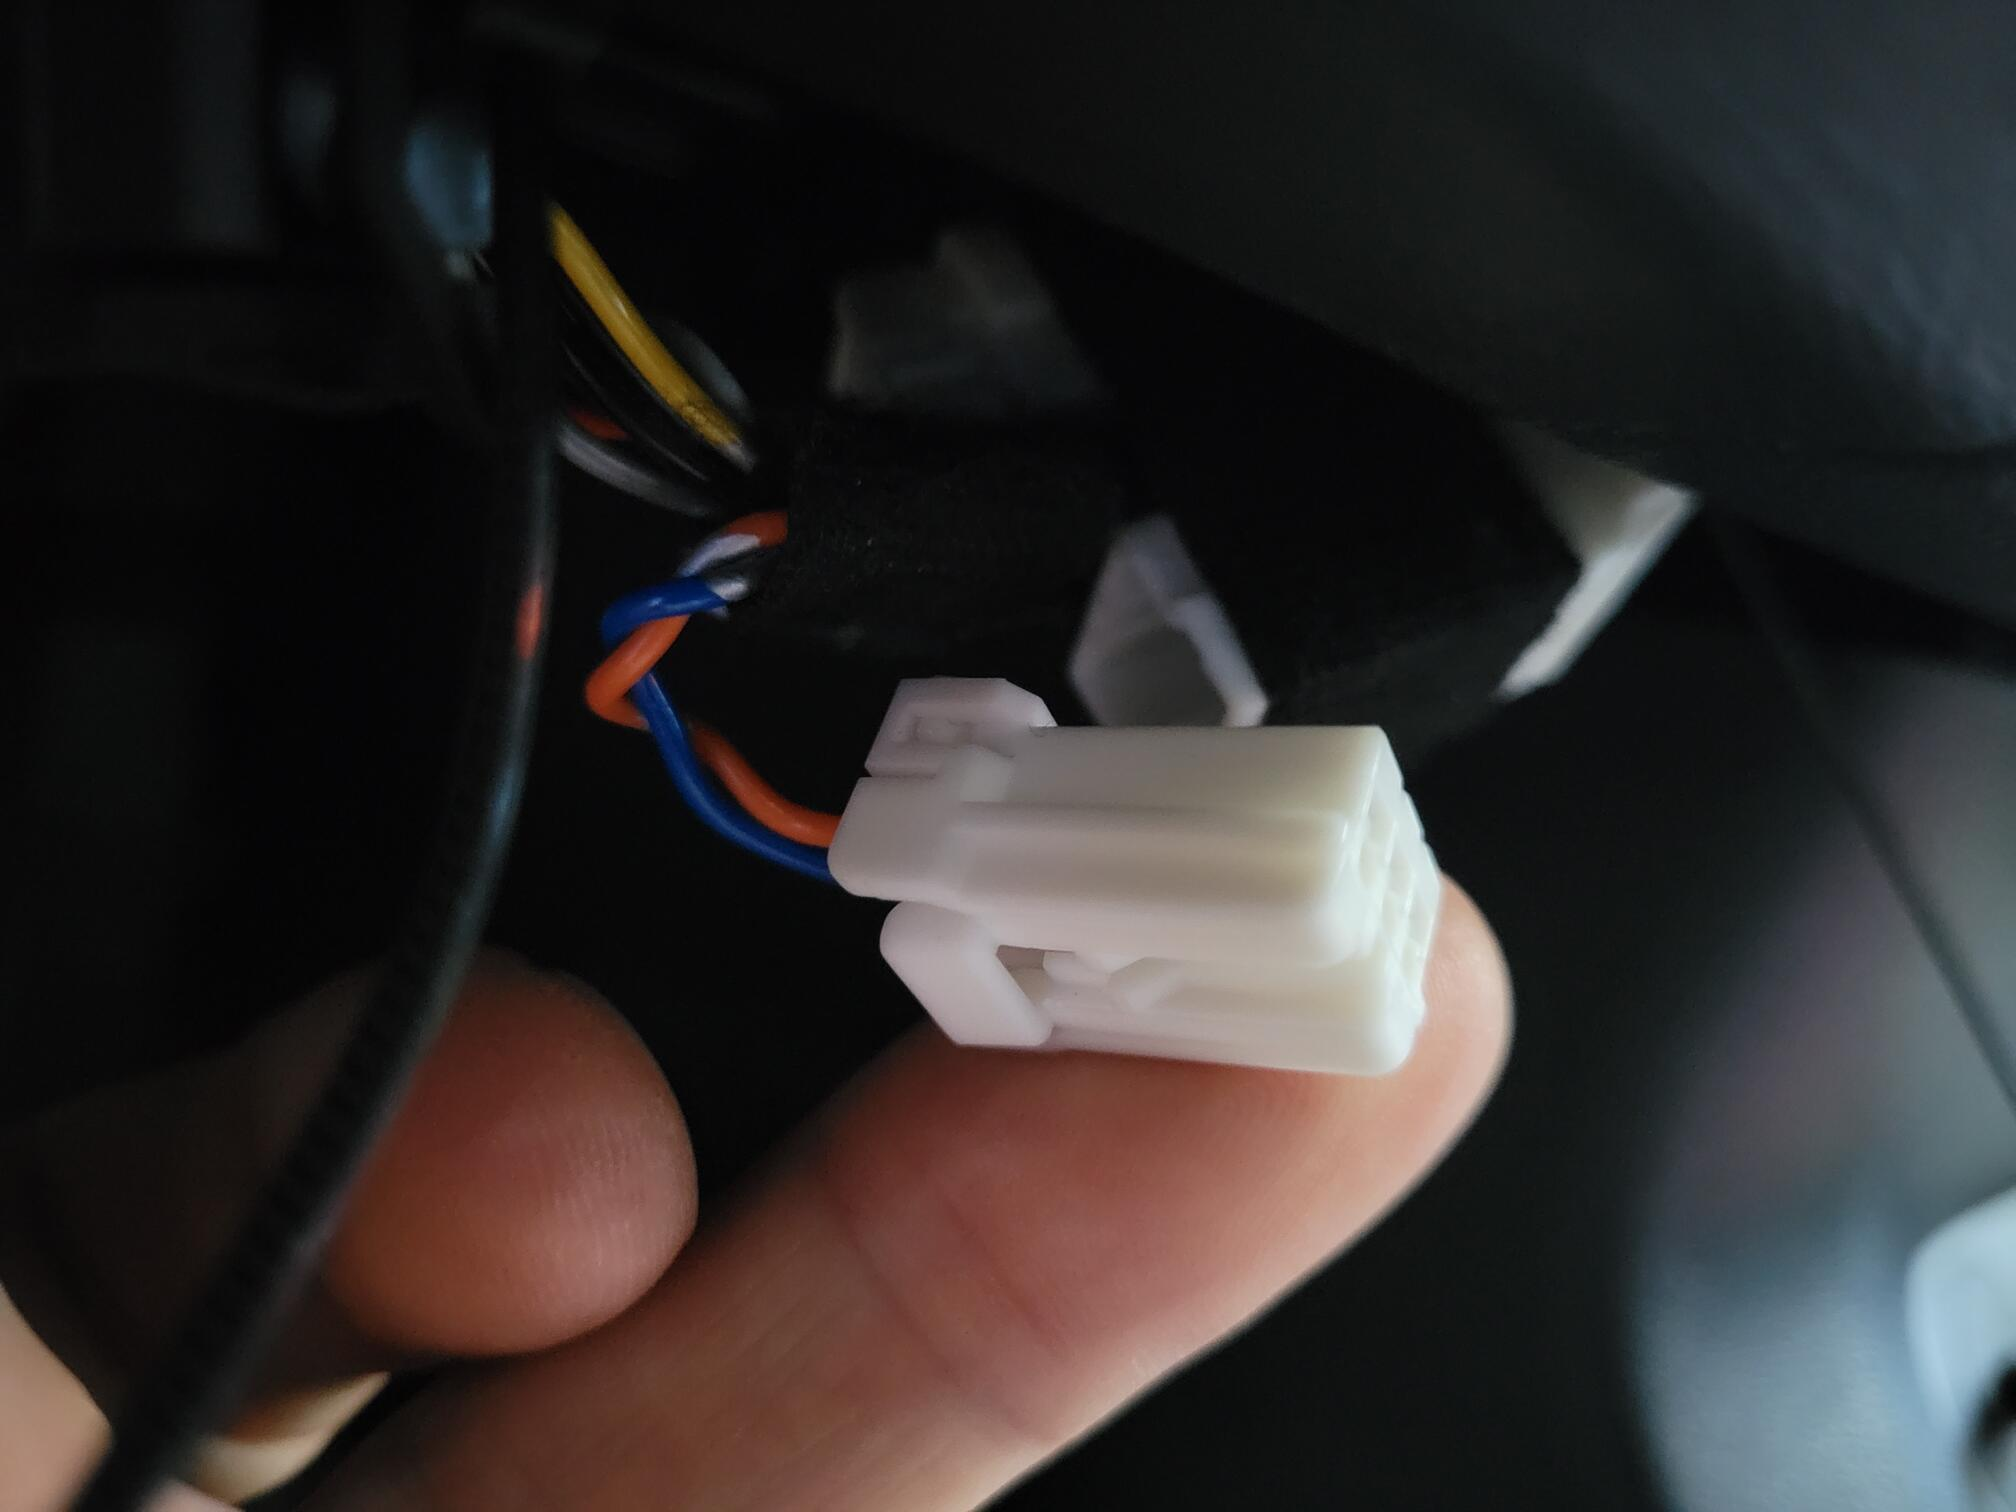
\includegraphics[height=0.95in]{photos/female_shunt_disconnected.jpg} } \\
  \subfloat[]{\label{subfig:shunt:cap_removed}
  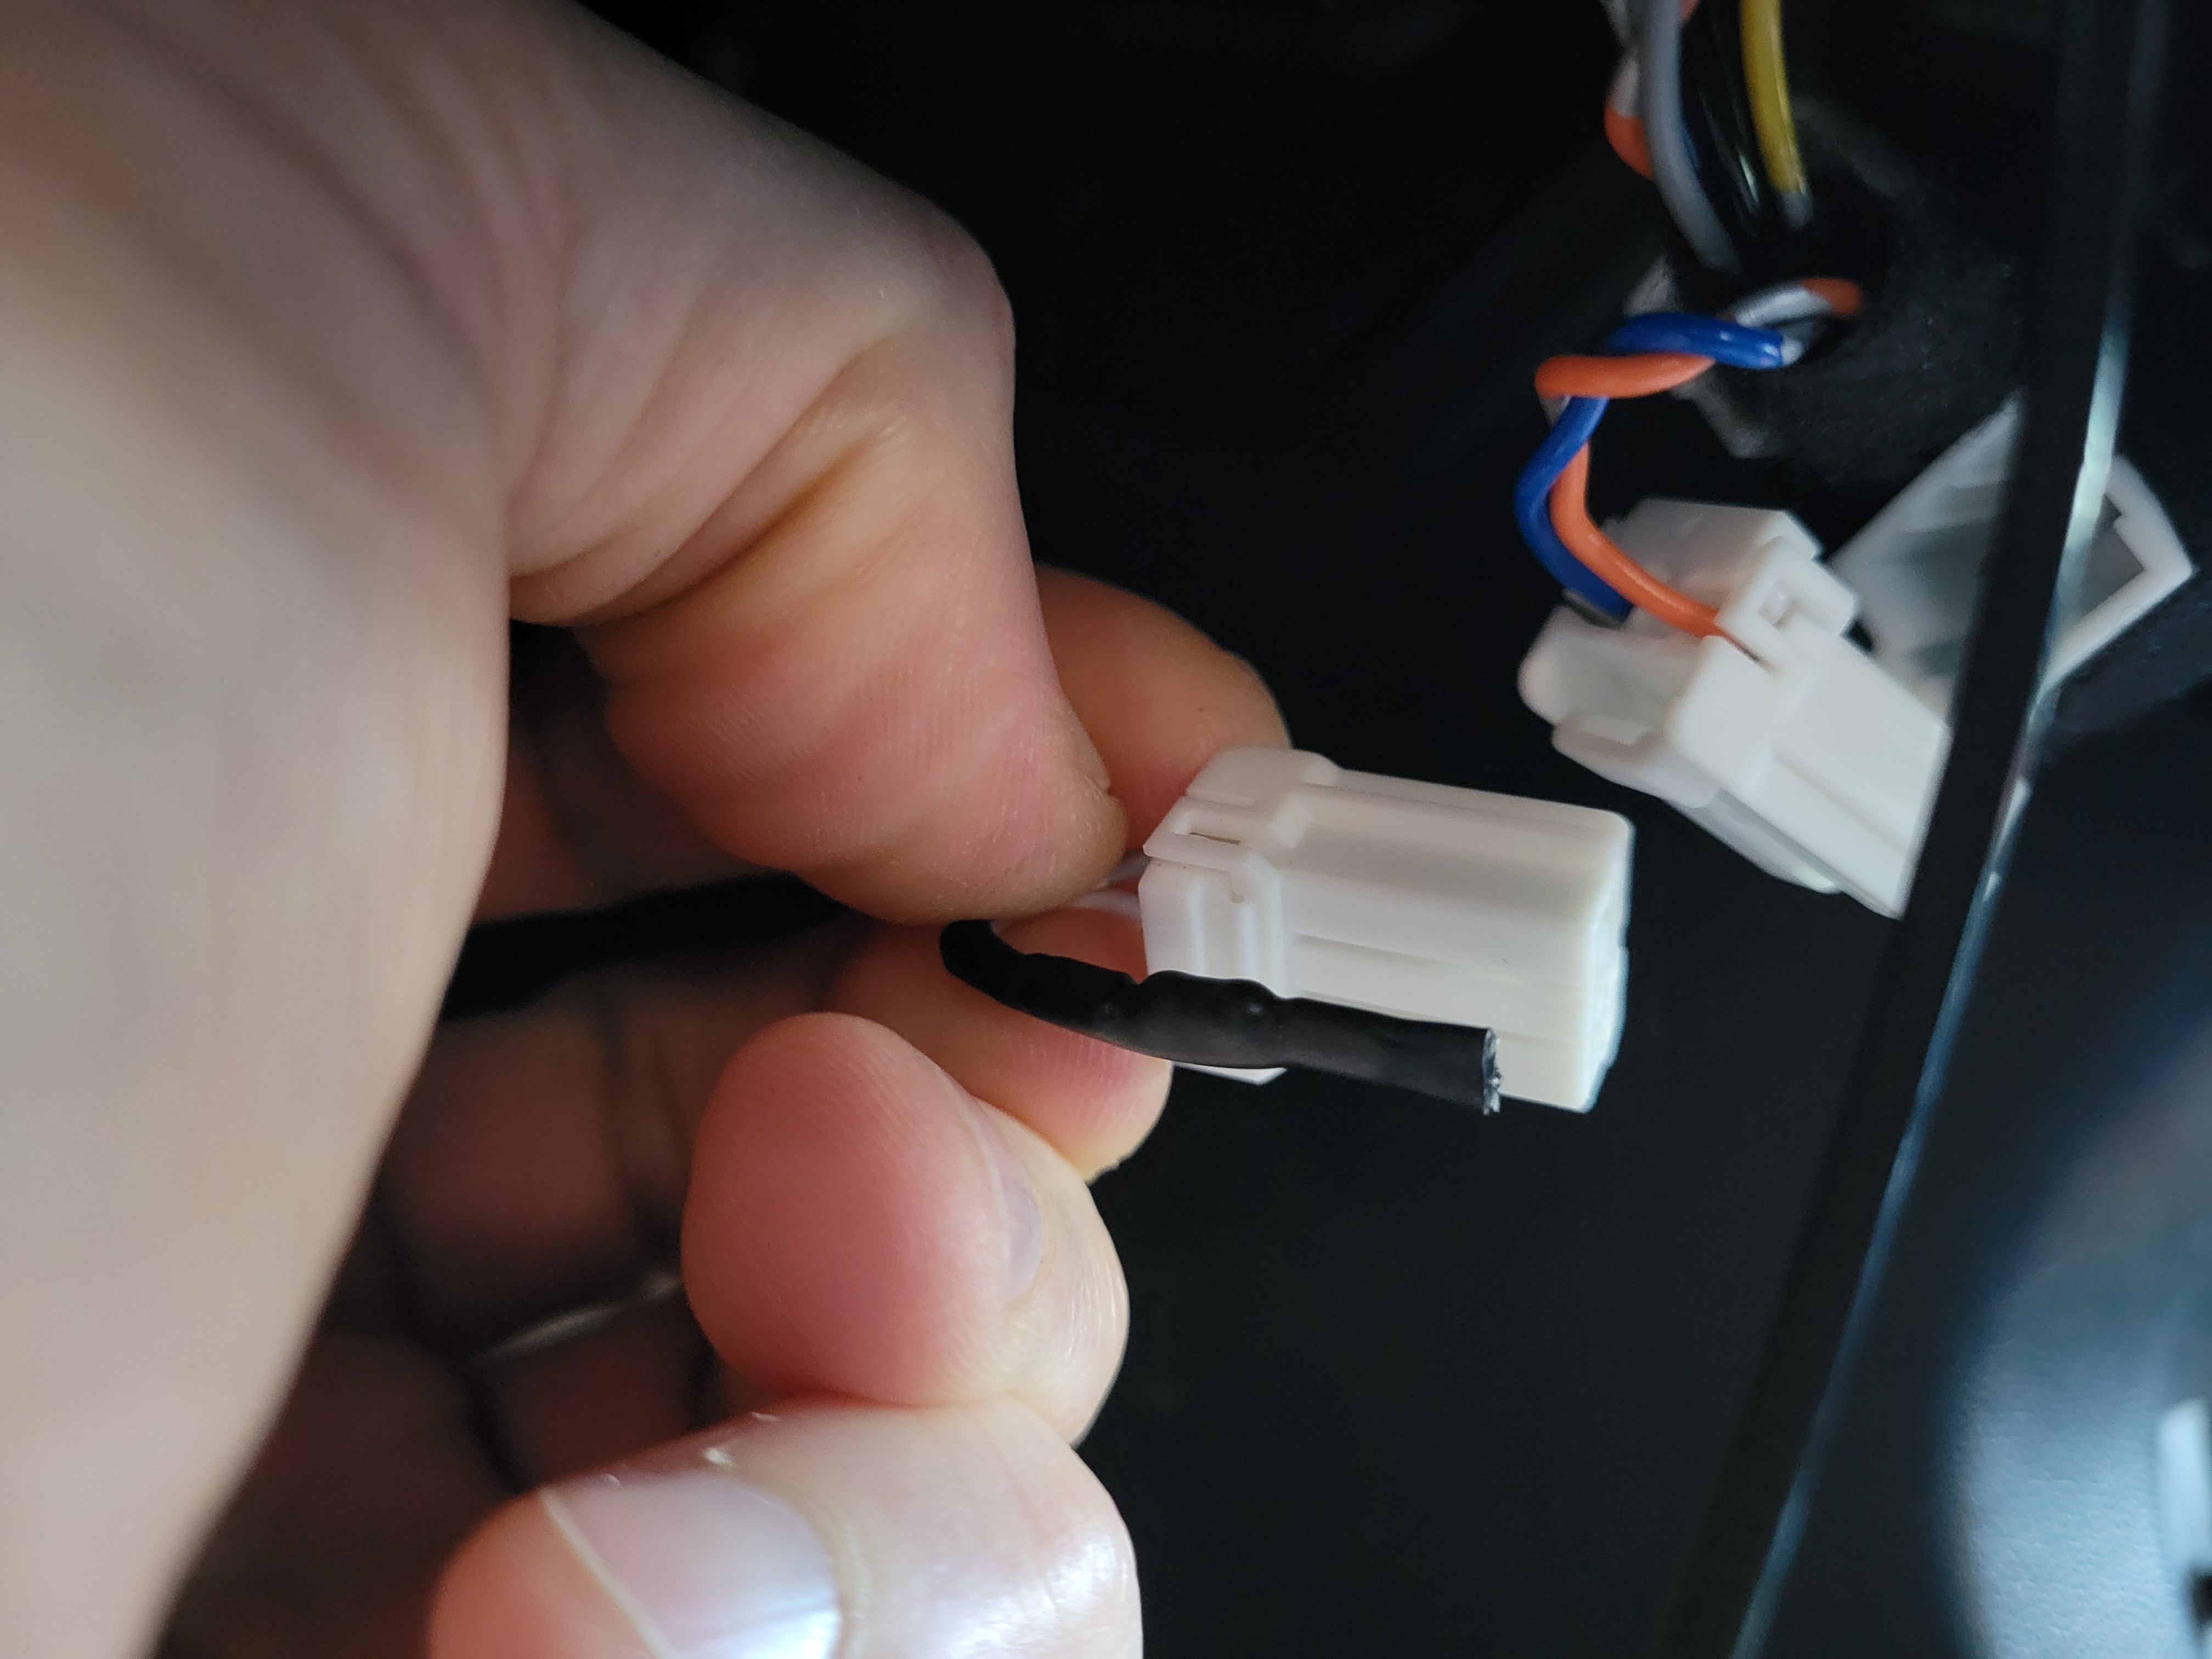
\includegraphics[height=0.95in]{photos/cap_removed.jpg} }
  \subfloat[]{\label{subfig:shunt:parallel}
  \includegraphics[height=0.95in]{photos/parallel.jpg} }
   \caption{(a-b) Female shunt cap: initial MITM mpde. (c) Disconnecting female shunt. (d) Disconnecting female shunt cap. (e) Parallel mode. \label{fig:shunts}}
\end{figure}
% %   \includegraphics[width=1.8in]{full_grating_nocblabel.png} }
% %   \begin{minipage}{1.5in}
% %     \vspace{-0.6in}
% \section{Experiment}
% 
% \begin{figure}[h]
%   \subfloat[]{\label{subfig:comparison:amp12}
%   \includegraphics[height=0.95in]{Capture12_amp_corrected_with_own_vacuum.png} }
%   \subfloat[]{\label{subfig:comparison:phase12}
%   \includegraphics[height=0.95in]{Capture12_phase_corrected_with_own_vacuum_labeled.png} }
%   \subfloat[]{\label{subfig:comparison:haadf12}
%   \includegraphics[height=0.95in]{Capture12_HAADF.png} } \\
%   \subfloat[]{\label{subfig:comparison:amp17}
%   \includegraphics[height=0.85in]{Capture17_amp_corrected_with_own_vacuum.png} }
%   \subfloat[]{\label{subfig:comparison:phase17}
%   \includegraphics[height=0.85in]{Capture17_phase_corrected_with_own_vacuum_labeled.png} }
%   \subfloat[]{\label{subfig:comparison:haadf17}
%   \includegraphics[height=0.85in]{Capture17_HAADF.png} } \\
%   \subfloat[]{\label{subfig:comparison:lacey_lineplot}
%   \includegraphics[height=1.1in]{STEMh-HAADF_comparison_lacey_carbon.png} }
%   \subfloat[]{\label{subfig:comparison:CdTe_lineplot}
%   \includegraphics[height=1.1in]{STEMh-HAADF_comparison_CdTe_noinset.png} }\\
%   \caption{Comparison of micrographs recorded by STEMH and ADF-STEM on lacey carbon and semidconducting nanoparticles. (a,d) Amplitude measured by STEMH. (b,e) Phase measured by STEMH; line profiles in (g,h) are taken along the white arrow and averaged over the width of the box. (c,f) Simultaneously acquired ADF. (g) Comparison of phase (red) with ADF (blue) on lacey carbon edge. Inset: zoom-in to show noise levels. (h) Same as (g) on the edge of a semiconducting nanoparticle. \label{fig:comparison}}%Inset: zoomed-in plot of the vacuum region just outside the particle. The phase outside the particle is fit well by an exponential decay (green). \label{fig:comparison}}
%   % starting at the edge of the particle, as determined by the maximum gradient of the ADF. 
% \end{figure}
% 
% 
\appendix 
\bibliographystyle{apsrev4-1}
\bibliography{stemh_model}{}
\end{document}
